\subsection{Camp Infrastructure}

Dreki (shown in Figure~\ref{figure:dreki_panorama}) is a small collection of buildings,
forming a semi-rugged campsite about 5 km east of Lake Askja.
It has 2 full cabins with rooms and bathrooms, 1 A-shaped cabin with a loft (no bathroom),
1 public bathroom, a reception, a building for the wardens and emergency workers,
and a large open area for tent camping.
We were not planning to stay in the cabins, as they are quite expensive.
So, the entire RAVEN team set up in the tent area,
with a set of large tents forming designated common spaces.
The personal tents were centered around ``Electric Avenue'' -- a designated place where our
fiber optic cable ran, in order to provide a private internet connection for the team.
This connection was primarily for data transfer from the field to offsite workers in Pasadena,
but was otherwise freely usable by all of us.
The solar array in Figure~\ref{figure:common_tents}
provided charge to 2 batteries in the shipping container,
which in turn provided US wall power (120 V) to the camp.
We used the public bathroom building for bathrooms, showering, and faucets for running water
which came from the nearby stream.

\begin{figure}
	\centering
	\includegraphics[width=\textwidth]{./images/dreki.jpg}
	\caption{Panorama of Dreki, centered east.}
	\label{figure:dreki_panorama}
	\includegraphics[width=\textwidth]{./images/common_tents.jpg}
	\caption{The tent area, with (left to right) our shipping container, solar panel array,
	4 common tents, and kitchen tent. The personal tents are in the background.}
	\label{figure:common_tents}
	\includegraphics[width=\textwidth]{./images/personal_tents.jpg}
	\caption{The tent city of the early group sent to prepare camp, taken on top of the future Electric Avenue.}
	\label{figure:personal_tent_city}
\end{figure}
\begin{figure}
	\centering
	\begin{subfigure}{0.49\textwidth}
	\includegraphics[width=\textwidth]{./images/personal_tent_inside.jpg}
		\caption{Inside of my personal tent. This held my 3 bags, 2 air mattresses
		(for thermal insulation against the cold ground), and 2 pillows.}
	\label{figure:personal_tent_inside}
	\end{subfigure}
	\centering
	\begin{subfigure}{0.49\textwidth}
	\includegraphics[width=\textwidth]{./images/kitchen_tent_inside.jpg}
	\caption{The kitchen tent, replete with tons of fruit, vegetables, tea, coffee, candy, etc. This was the domain of our wonderful chef Guðrún.}
	\label{figure:kitchen_tent}
	\end{subfigure}
\end{figure}

\subsection{Weather}

The weather at Dreki is not to be underestimated, and indeed proved multiple times to be a challenge.
On a normal day, the temperature ranged from about
$8^\circ \mathrm{C}=46^\circ \mathrm{F}$ to $12^\circ \mathrm{C}=54^\circ \mathrm{F}$,
with occasional extremes of freezing or up to $15^\circ \mathrm{C}=59^\circ \mathrm{F}$.
It also rained at least half of the days (maybe more), sometimes for prolonged periods.
Windstorms with gusts well over 25 m/s destroyed some larger tents, deformed smaller tents,
and ultimately forced most of the tent inhabitants to move into one of the cabins.
The 4-person Mountain Hardware tents, among others, handled the wind the best.
It is \emph{necessary} to bring the proper clothing and equipment
(such as in the following non-exhaustive list), and to not underestimate the weather:
\begin{itemize}
	\item \textbf{Wool or synthetic base layers}\\(top and bottom)
	\item \textbf{Wool socks}\\I wore cotton ankle socks (as liners to keep the wool socks cleaner for longer) inside wool, full-length,
		waterproof socks (SealSkin).
	\item \textbf{Waterproof external layers}\\It is good to have GoreTex shells
		as external pants and jackets.
	\item \textbf{Waterproof gloves}\\Gloves are necessary, and with the amount of rain it is much
		more comfortable to have waterproof ones.
	\item \textbf{Cold-weather sleeping bag}\\Rated for temperatures significantly below freezing.
	\item \textbf{Sleeping bag liner}\\To keep the sleeping bag clean and increase its heat retention.
	\item \textbf{A \emph{small}, cold-weather tent}\\Larger tents cannot handle the wind and may be destroyed. This is not an exaggeration. It actually happened. A ``blackout room'' can help with sleeping in the never-ending summer brightness.
	\item \textbf{Sand screws}\\Normal, straight tent stakes do not work in this terrain. It is better to use something that cannot be removed from the soft, rocky ground by pulling it up vertically. Sand screws should be installed such that its guideline pulls at roughly a $90^\circ$ angle from its axis.
\end{itemize}

It may snow in the summer at Dreki, and indeed did snow during the fieldwork in 2022,
as shown in Figure~\ref{figure:snow}.

\begin{figure}
	\centering
	\begin{subfigure}{0.49\textwidth}
	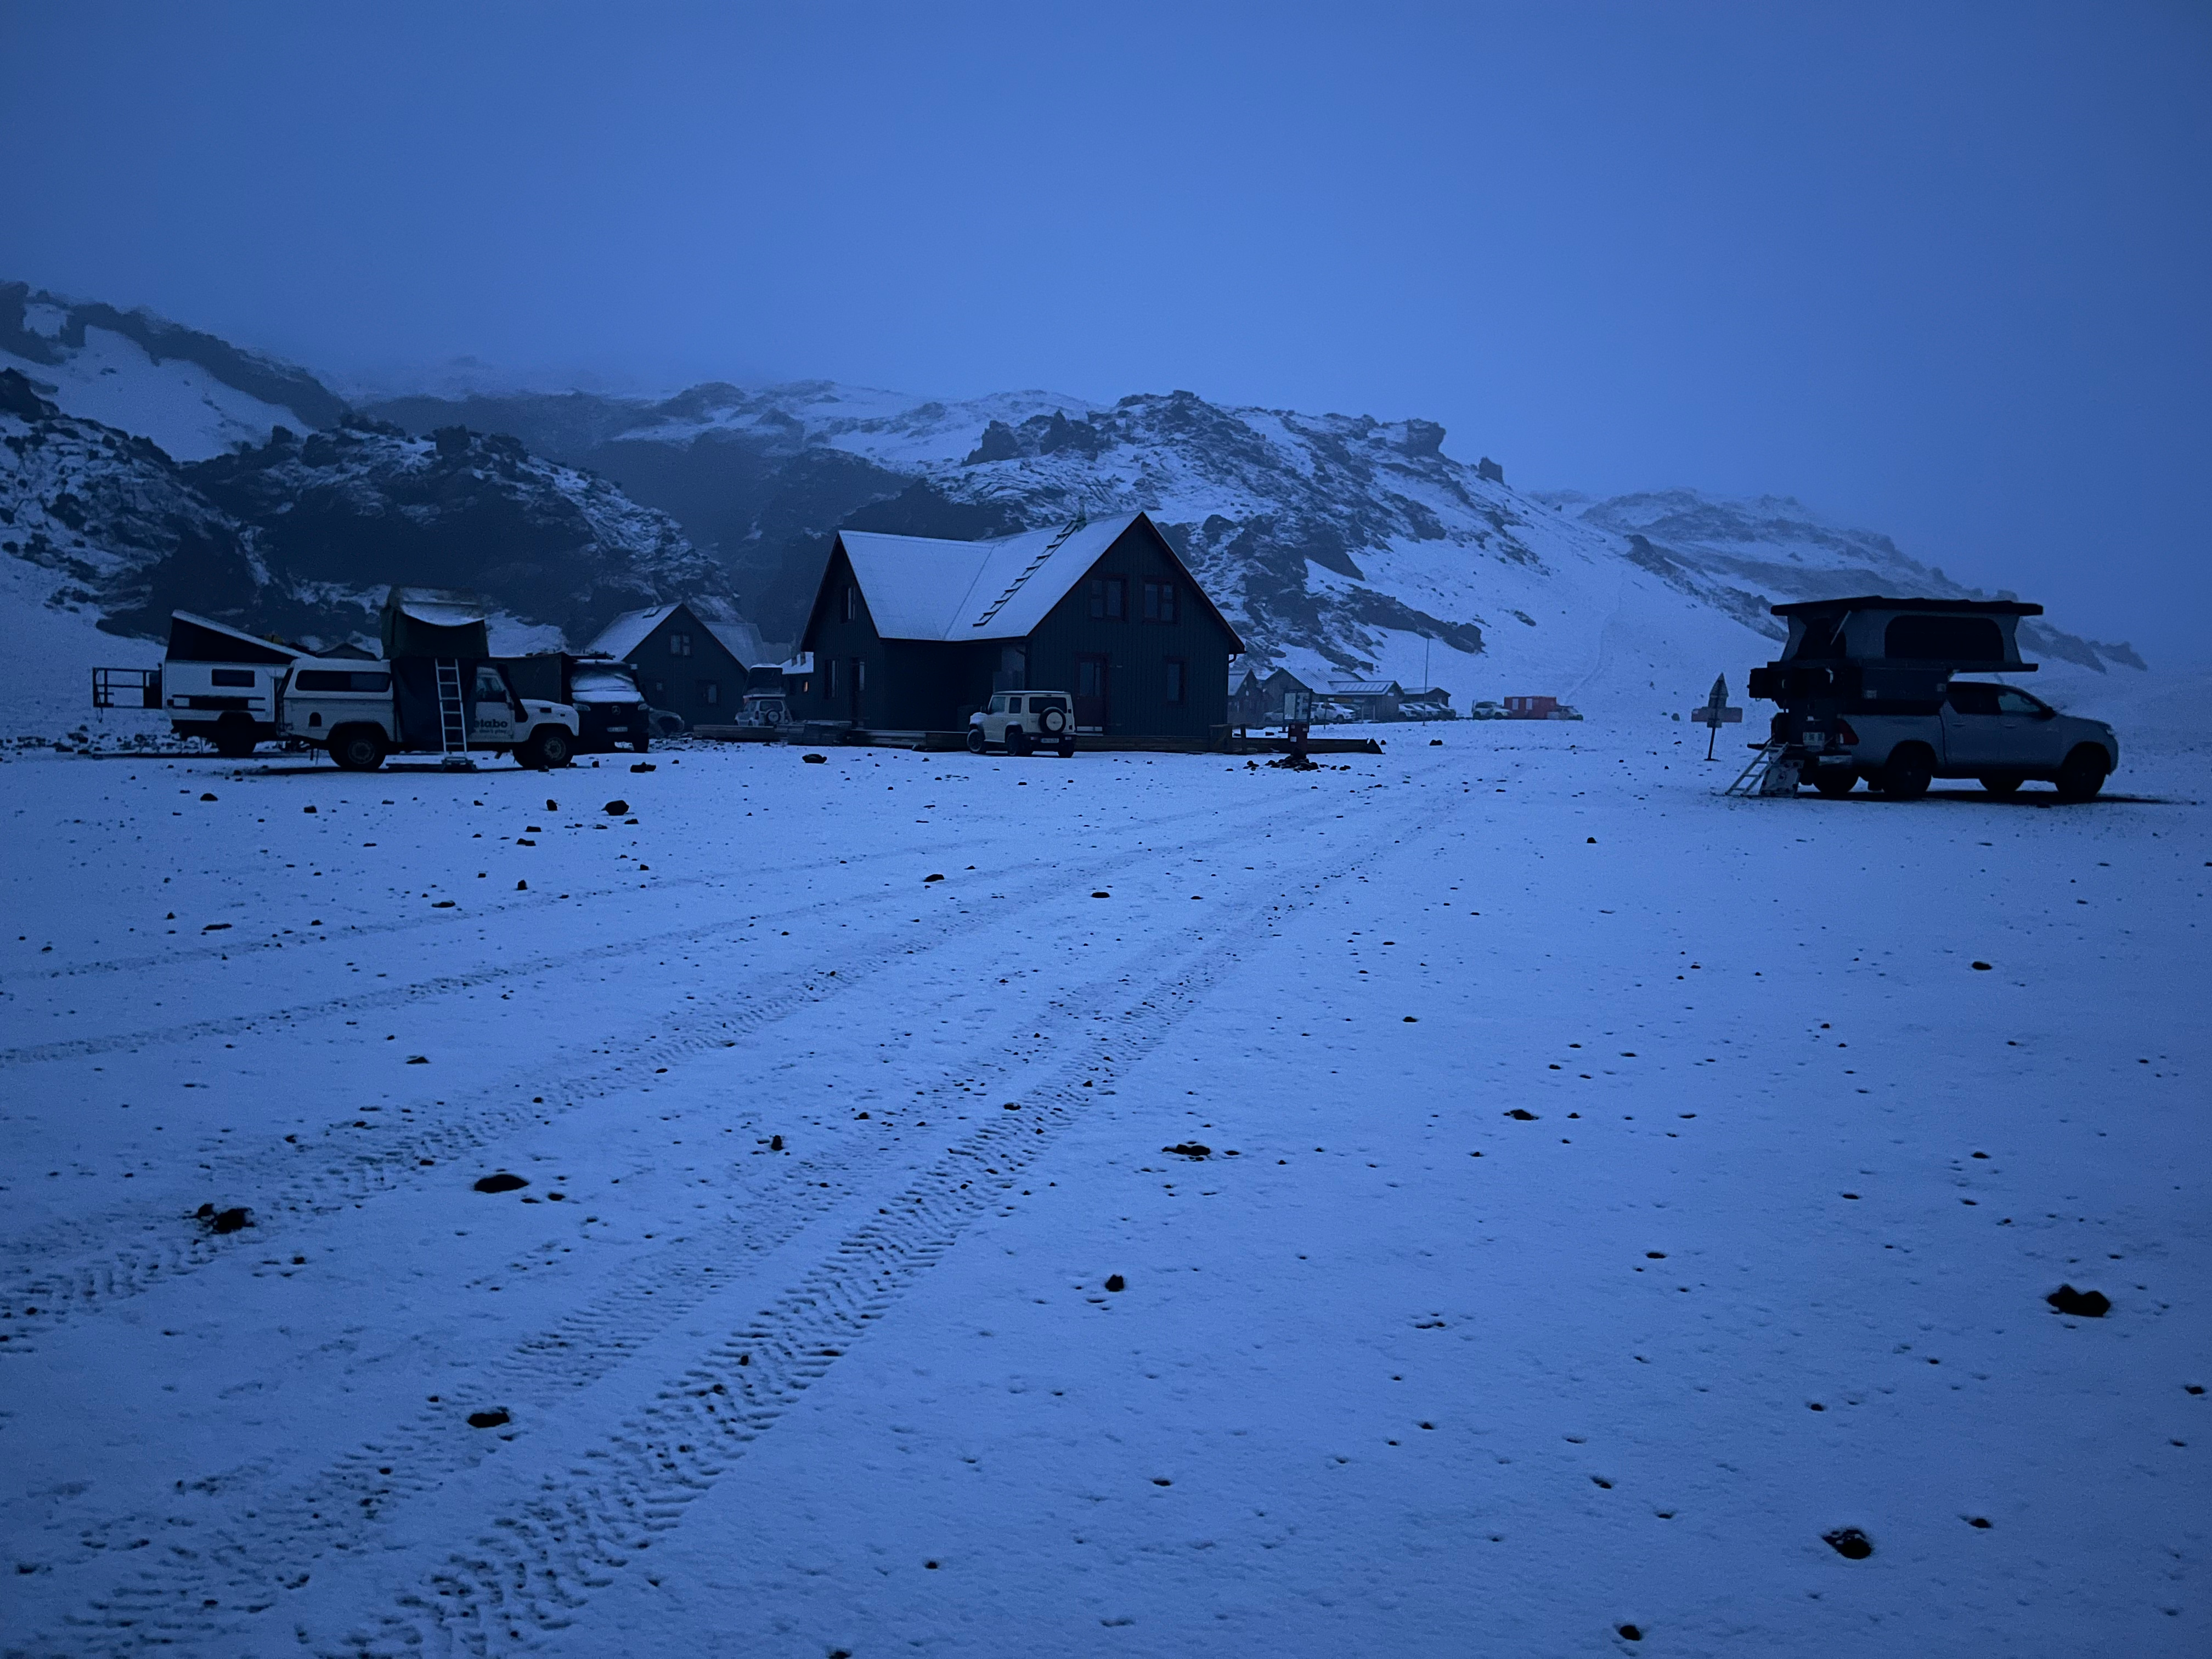
\includegraphics[width=\textwidth]{./images/snow_dreki.png}
		\caption{Dreki with snow.}
	\label{figure:snow_dreki}
	\end{subfigure}
	\centering
	\begin{subfigure}{0.49\textwidth}
	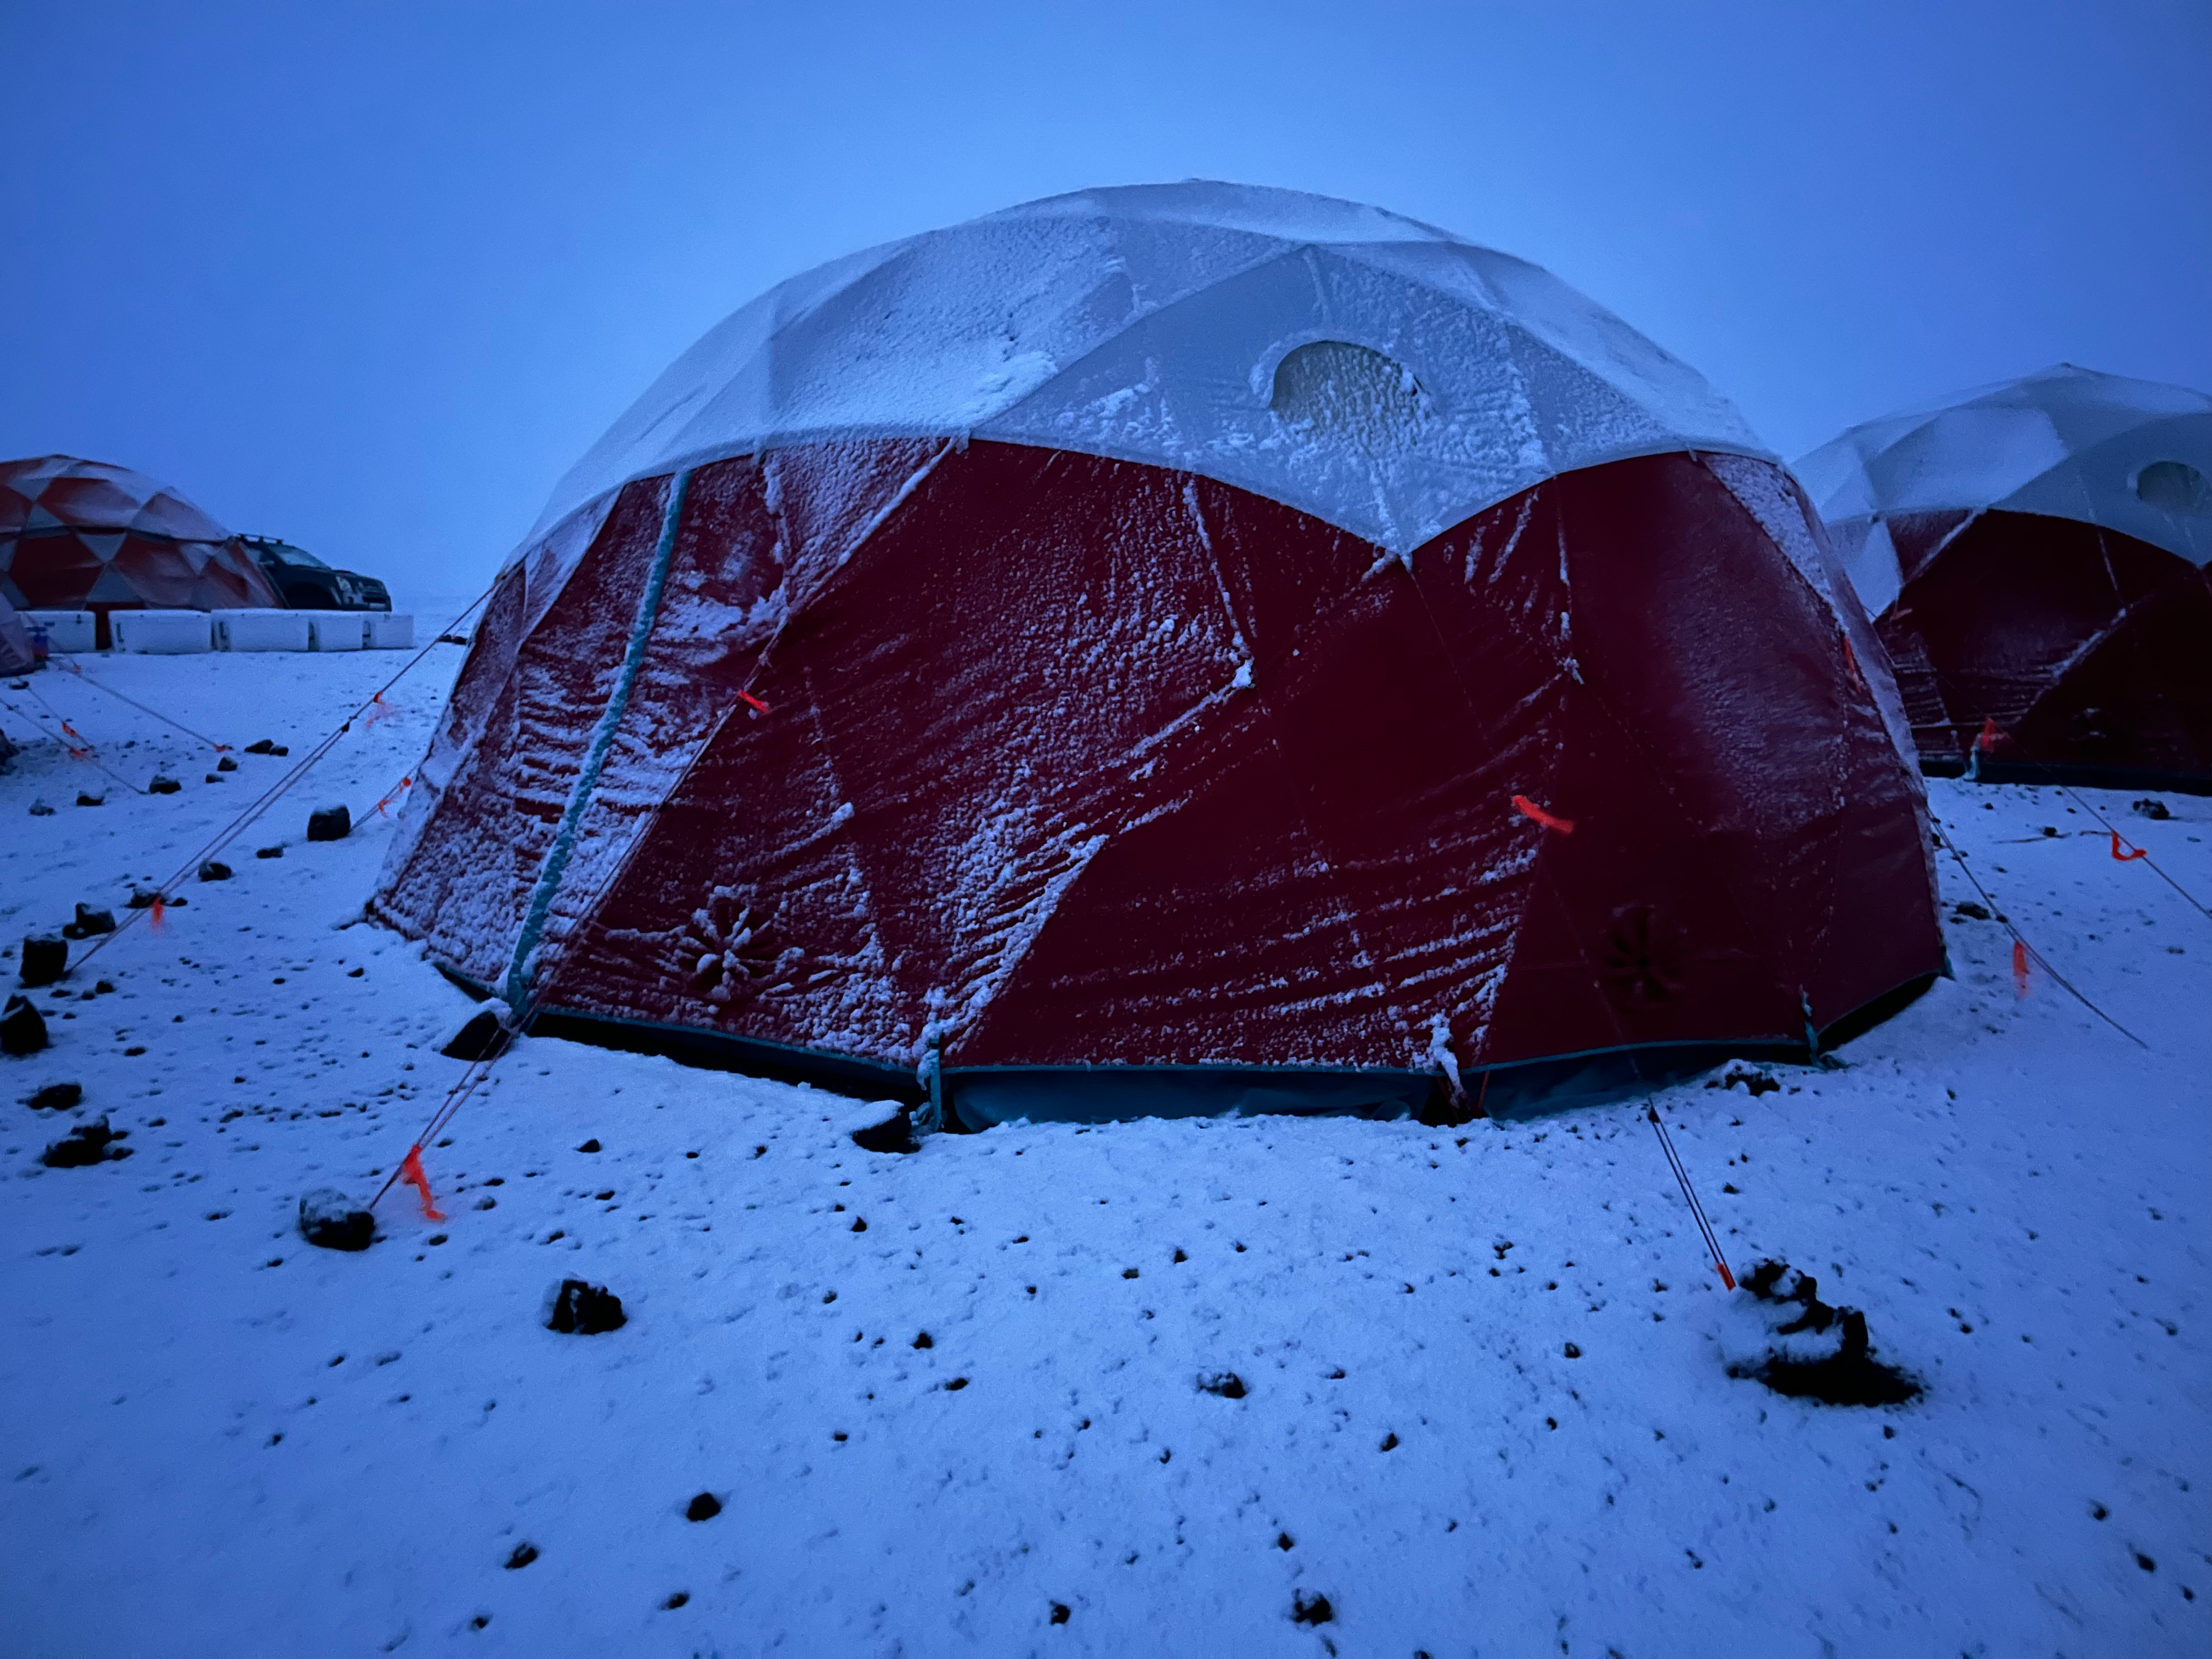
\includegraphics[width=\textwidth]{./images/snow_big_tent.png}
	\caption{Space station tent with snow.}
	\label{figure:snow_space_station_tent}
	\end{subfigure}
	\begin{subfigure}{0.49\textwidth}
	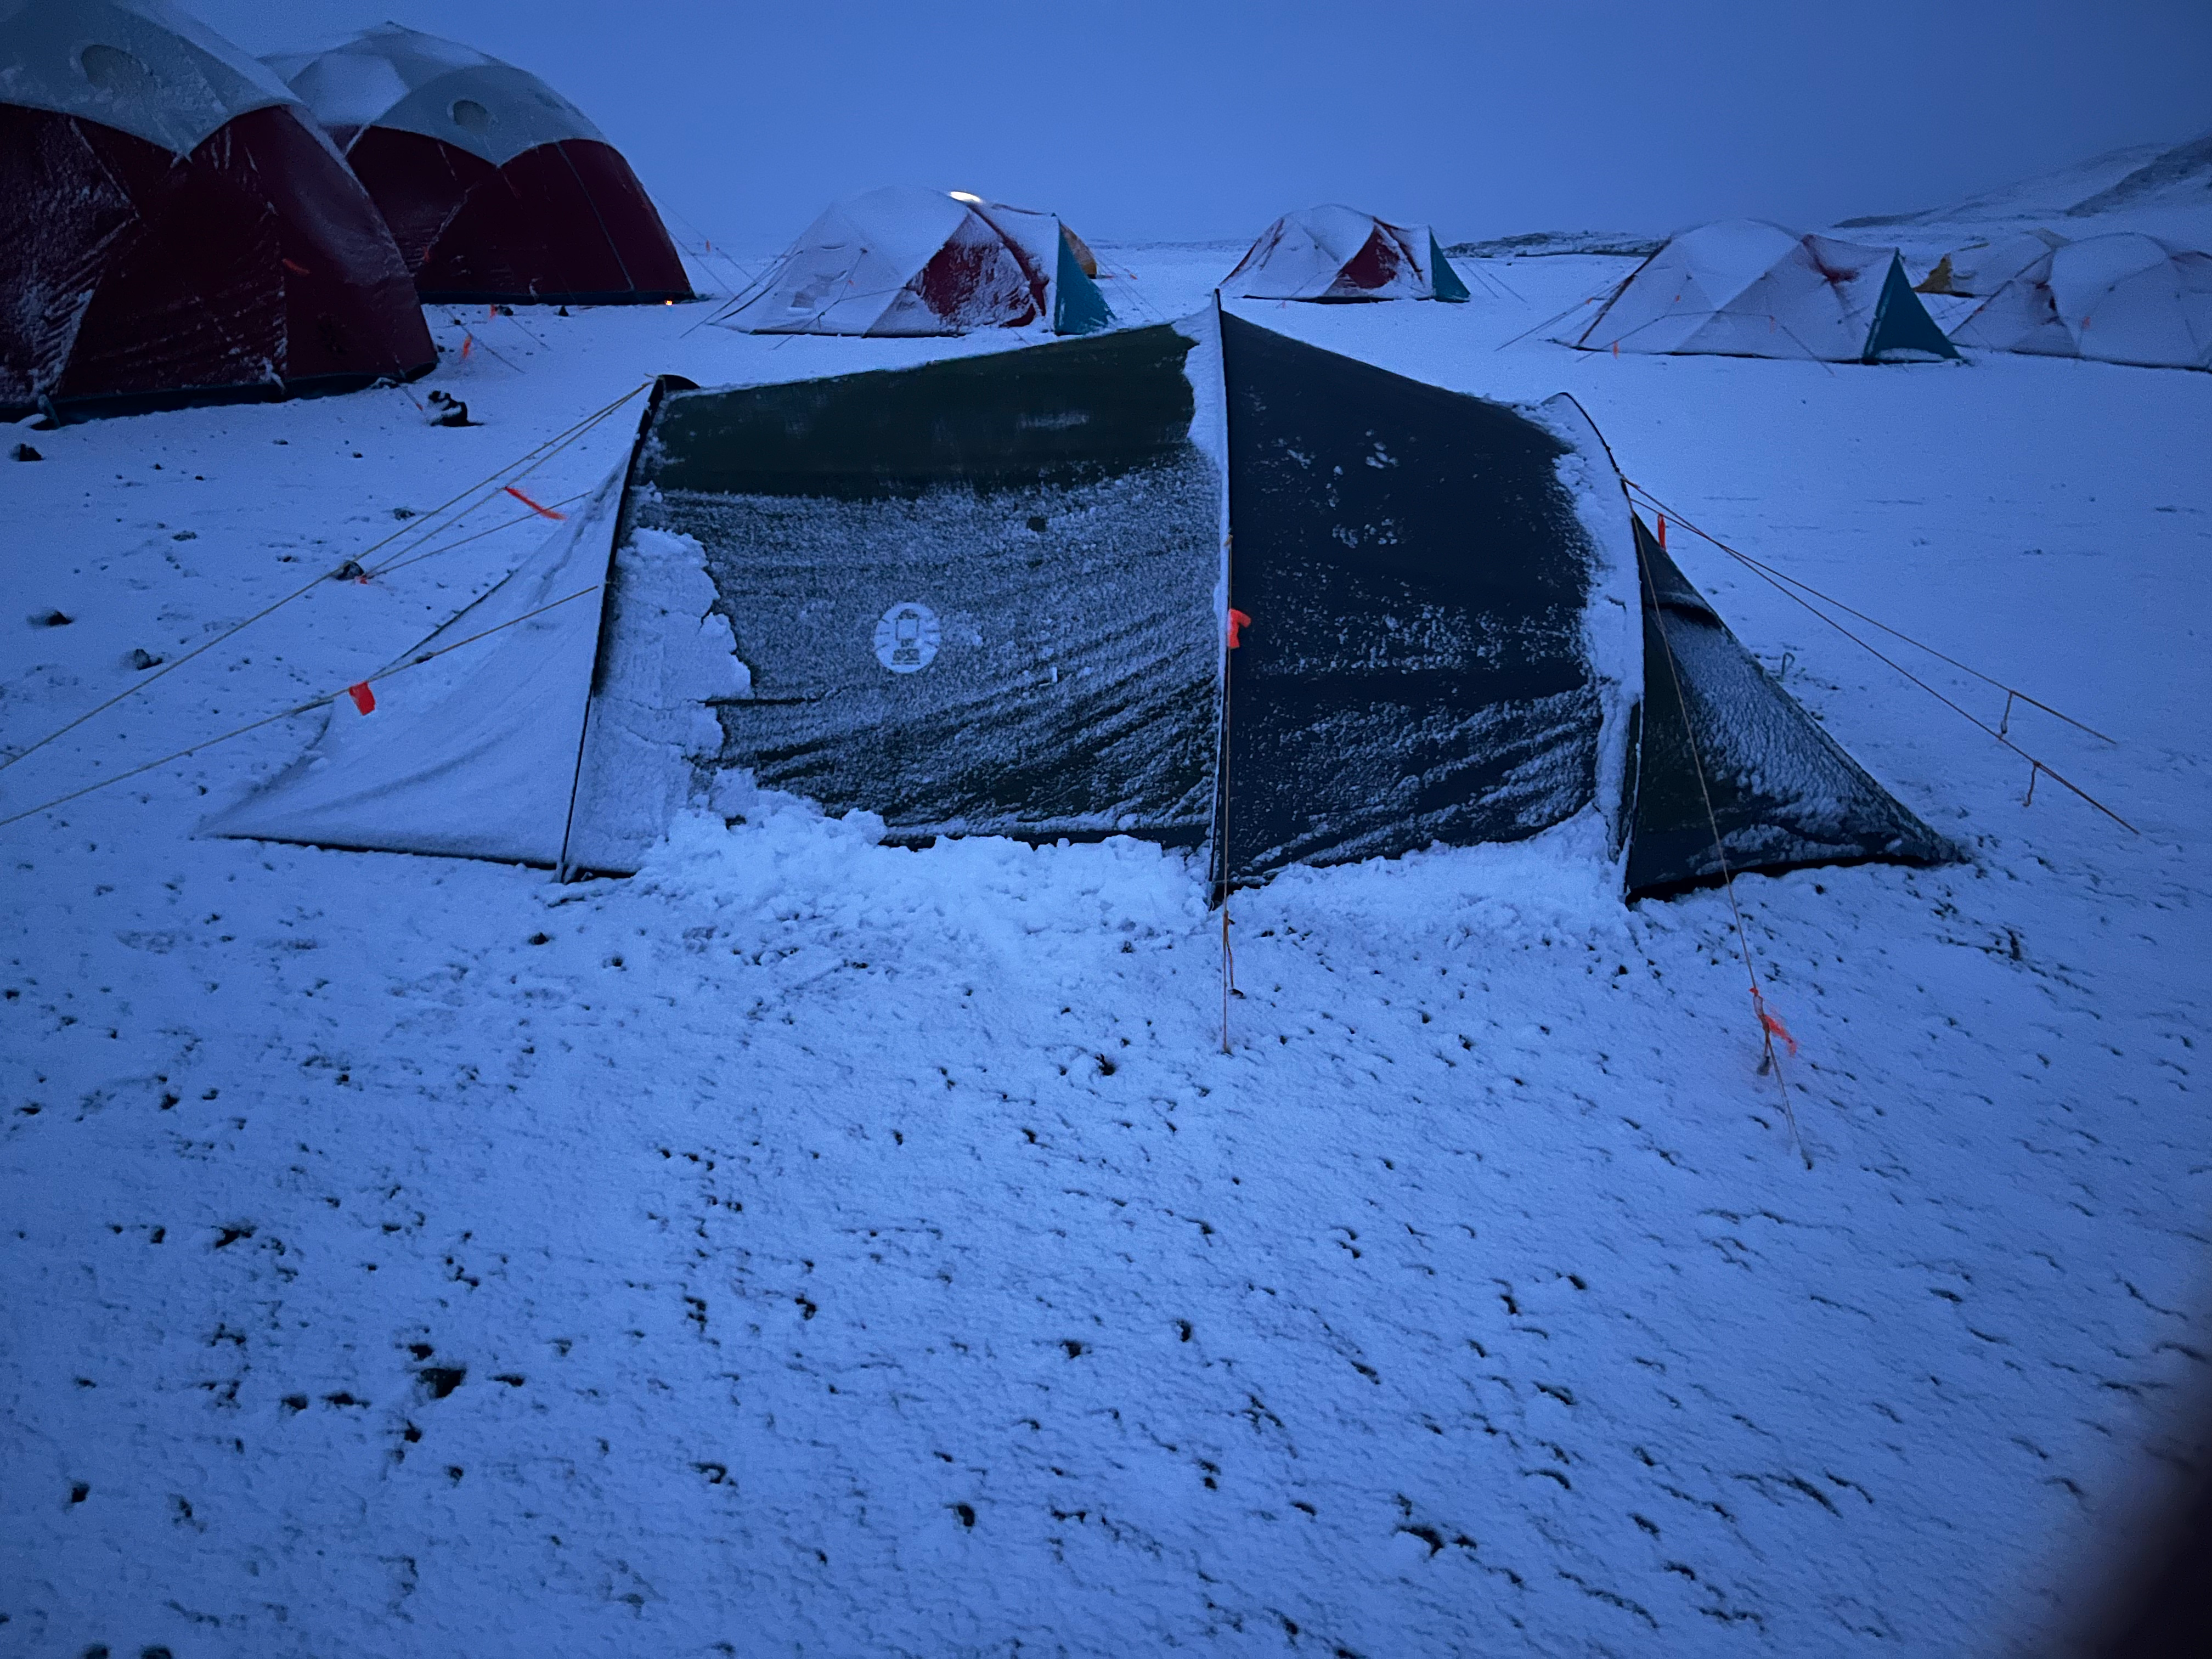
\includegraphics[width=\textwidth]{./images/snow_small_tent.png}
	\caption{Personal tent with snow.}
	\label{figure:snow_personal_tent}
	\end{subfigure}
	\caption{Sudden, non-negligible summer snow event.}
	\label{figure:snow}
\end{figure}

